
\documentclass[final,5p,twocolumn]{elsarticle}

\usepackage{graphicx}
\usepackage[usenames]{color}
\usepackage{multirow}
\providecommand{\note}[1]{\textcolor{red}{\textbf{ #1 }}}

\journal{Computers \& Graphics}

\begin{document}
\begin{frontmatter}
\title{The Effect of Task on Classification Accuracy: Using Gesture Recognition Techniques 
      in Free-Sketch Recognition}

\author[hmc]{M.~Field}
\ead{mfield@cs.hmc.edu}

\author[hmc]{S.~Gordon}
\author[ucr]{E.~Peterson}
\author[hmc]{R.~Robinson}

\author[ucr]{T.~Stahovich}
\ead{stahov@engr.ucr.edu}
\author[hmc]{C.~Alvarado}
\ead{alvarado@cs.hmc.edu}

\address[hmc]{Harvey Mudd College, Department of Computer Science, Claremont, California}
\address[ucr]{University of California: Riverside, Department of Mechanical Engineering, Riverside, 
California} 

\begin{abstract}
Generating, grouping, and labeling free-sketch data is a difficult and
time-consuming task for both user study participants and
researchers. To simplify this process for both parties, we would like
to have users draw isolated shapes instead of complete sketches that
must be hand-labeled and grouped, and then use this data to train our
free-sketch symbol recognizer.  However, it is an open question
whether shapes drawn in isolation accurately reflect the way users draw
shapes in a complete diagram.  To answer this question, 
we present a systematic exploration
of the effect of task on recognition accuracy using three different recognizers.
Our study examines how task affects accuracy in the context of 
user-independent, user semi-dependent
and user-dependent training data.   We find that as the amount of 
user-specific training data increases, the effect of task on recognition 
accuracy also increases.  We also show that the best overall recognition 
results are obtained by using user semi-dependent, task-specific training data.  
These results hold across three different domains: circuit diagrams, entity
relationship diagrams and process diagrams.  Finally,
we introduce a variant of a popular and simple gesture recognition
algorithm that recognizes freely-drawn shapes as well as a
highly-accurate but more complex recognizer designed explicitly for
free-sketch recognition.

%\begin{classification} % according to http://www.acm.org/class/1998/
%\CCScat{Information interfaces and presentation}{H.5.2}{User Interfaces}{Interaction styles}
%\CCScat{Pattern recognition}{I.5.2}{Design methodology}{Classifier design and evaluation}
%\CCScat{Pattern recognition}{I.5.5}{Implementation}{Interactive systems}
%\end{classification}

\end{abstract}

\begin{keyword}
Interaction styles \sep Classifier design and evaluation \sep Interactive Systems
\end{keyword}

\end{frontmatter}

%-------------------------------------------------------------------------
\section{Introduction}
Having realistic training data is essential to developing robust
recognition algorithms.  Obtaining such data for sketch recognition 
can be an arduous process. Public data sets are
emerging~\cite{oltmans04,hse05,wolin07,paulson08,blagojevic08}, but these
necessarily represent a limited number of domains and often include
only shapes drawn in isolation, rather than complete sketches.

Many of the most robust and complete sketch recognition systems today
(e.g. \cite{zeleznik08} and~\cite{lee08}) focus
on gesture or isolated symbol recognition rather than the more
difficult problem of free-sketch recognition.  Such systems constrain
users to draw shapes one at a time, avoiding the considerable
difficulties of finding the boundaries between them.  Gesture
recognition often additionally constrains the user to draw each shape
with a specific style (e.g., users might be required to draw
rectangles with a single clockwise pen stroke).

Because of these simplifications, collecting training data for gesture
recognizers is (relatively) straightforward.  Users can be prompted to
draw each gesture individually, without need for any manual processing
or labeling.  Because of the limited variation in drawing style, a
recognizer trained on data from one set of users is likely to work
well for other users. Additionally, many gesture recognition
algorithms (e.g.~\cite{wobbrock07}) can be fine-tuned for an individual
user by simply having them draw a few examples.

Obtaining training data for free-sketch recognition systems is
considerably more difficult than for gesture-based systems. In recent
years, researchers have developed several tools to facilitate the
collection and labeling of data
\cite{wolin07,paulson08,blagojevic08}.  However,
even with these tools, processing the data is still a labor- and
time-intensive task because the pen strokes must be manually grouped
into individual symbols and labeled.  Furthermore, most of these tools
are designed for researchers. It would be impractical for an end-user
to manually group and label the symbols in a freely drawn sketch to improve a
system's recognition performance.


For these reasons, researchers frequently obtain recognition training
data for free-sketch recognition systems using the same simplified
data collection process suitable for gesture-based systems (e.g.,
\cite{kara05,hse04}). In the current work, we seek to
evaluate the soundness of this approach, explicitly examining the usefulness
of symbols drawn in isolation for training shape recognizers for
free-sketch recognition.  The answer to this question is not obvious,
as drawing isolated symbols is not the same as drawing them in the
context of a larger task. For instance, drawing a logic gate by itself
is substantially different from designing a digital circuit.  In the
former case, the user's focus is on the drawing task, while in the
latter, the user's focus is likely to be the \textit{design} task.  
It is possible that this difference in focus affects the way that 
the user draws the gate in question.

In this work, we quantitatively assess how much drawing task affects recognition 
accuracy in order to inform the design of free-sketch recognition 
systems.  We obtained two data sets in which users were asked to perform
sketching tasks of varying complexity.  In the first set (which we gathered
ourselves) participants were asked to draw logic gates
in isolation, to copy digital circuits, and to synthesize and sketch new
circuit designs.  In the second set (from~\cite{schmieder09}), participants
were asked to draw basic shapes such as rectangles and lines in isolation, 
and to draw entity relationship diagrams and process diagrams (both
of which involve the basic shapes from the isolated drawing task).  
We then examined how recognition accuracy varies
with the task used to obtain training data.  We examined this 
question for several highly accurate recognizers, including a state of the
art symbol recognizer~\cite{kara05} and several 
new extensions to a popular gesture 
recognition algorithm~\cite{wobbrock07}. We also examined this question
in the context of three different training sets that included varying 
amounts of user-specific data.  

We show that for all recognizers, the sensitivity of the recognizer 
to the task users perform depends on the amount of user-specific 
training data used to train the recognizer.  When we train the 
recognizers on user-independent data, we find that 
that recognition accuracy is not highly dependent on the task
users performed when generating training data.  Simple isolated symbol
data works just as well for training symbol recognizers as symbols
extracted from complex sketches. However, we find that including user-specific examples
in the training process makes the recognizers sensitive to task: 
e.g. a recognizer trained on complex sketches will perform better
when recognizing complex sketches than a recognizer trained on isolated data.
Furthermore, including
user-specific examples in the training process gives a significant
boost to accuracy, though reasonably accurate recognizers
can be produced even without user-specific examples.  

Finally, we present a new variant of
the recently proposed and very popular \$1 recognizer~\cite{wobbrock07}
that works on freely-drawn shapes comprised of any number of strokes
drawn in any order.  Our new recognizer performs with
comparable accuracy to an existing algorithm designed specifically
for recognizing freely-drawn shapes.

%-------------------------------------------------------------------------
\section{Background}

The central focus of the present work is to determine if variations
in drawing task may lead to variations in 
drawing style, thus impacting symbol recognition accuracy.
Relatively few studies have examined how people
draw, especially across different tasks.  Oltmans et al.~present some preliminary observations
from sketches from multiple domains~\cite{oltmans04}.
Although collected in a laboratory, these sketches simulate natural
drawing style as users were asked to produce an original design rather
than copy an existing diagram or draw specific shapes.  Alvarado and
Lazzareschi analyze drawings made by students in a circuit design
class as part of their routine course work~\cite{alvarado07}.  
They find that drawing styles
vary across students and even across the sketches of a single student.  On
the other hand, Sezgin and Davis find that the order in which users draw
strokes is relatively consistent across users when they are asked
to repeatedly draw military course of action symbols in
isolation~\cite{sezgin07}.  Our study adds to this 
previous work by quantifying the amount
of drawing variation in circuit diagrams across task and the 
impact these variations have on recognition accuracy.

Others have focused on note-taking styles in general.
Shilman et al.~examine free-form
handwritten notes in detail, specifically focusing on identifying
structure and handwriting within these
notes~\cite{shilman03}, but they do not examine the
diagrams themselves. Anderson et al.~examine
diagrams created by professors while
lecturing~\cite{anderson05}, but again their work does not
focus on how people draw diagrams.

The work most similar to ours is the recent
study by Schmieder et al~\cite{schmieder09}.
They compared the performance of several single-stroke recognizers
on data collected from users drawing different types of diagrams.  Their results indicate 
that recognition performance differs depending on whether the test data was collected 
from an artificial or natural drawing task.  
Though while their results suggest differences, their experiments were not
designed to judge whether these differences were statistically significant.  
Their primary goal was to showcase their application for managing and running such studies.  They 
also did not investigate the effect of user-specific data in their training set.
As described below, we expand on their initial results by performing experiments with their dataset.
We find that differences in recognition accuracy are not generally 
statistically significant for user-independent
recognizers, but become significant (and the overall recognition rate 
increases) when the recognizers are trained with user-specific data.

  
Researchers have developed countless shape and gesture recognition
algorithms over the last few decades.  Some focus on shape
(e.g.~
\cite{hammond04,alvarado04,learned06,kara05,wobbrock07}
to name only a few) while others extract features from the shapes
(e.g.~\cite{blagojevic08,hse04,rubine91,fonseca02,lee06},
again to name only a few).  

In the field of gesture recognition, two
algorithms stand out as the most widely-used: the Rubine classifier \cite{rubine91}
and the recently proposed \$1 recognizer \cite{wobbrock07}.  The Rubine classifier, the
first widely used gesture recognizer, is a feature-based linear
classifier, while the \$1 recognizer is a nearest-neighbor classifier
that examines the locations of the sampled pen-strokes on a gesture.  
Compared to the Rubine classifier,
the \$1 recognizer has the advantage that users can easily train it to
match their drawing styles by drawing a few examples of each gesture.

In this paper we compare two extensions of the \$1 recognizer with a
robust image-based recognition algorithm for sketch recognition
presented in~\cite{kara05}.  This recognizer, also a
nearest neighbor classifier, has been shown to be one of the best at
recognizing symbols in the face of drawing style variations and also
can be easily adapted to an individual user by having the user draw a
few examples of each symbol.  We did not consider the Rubine recognizer
in our comparisons because of its extremely poor performance on 
our data sets in our initial tests.  

%-------------------------------------------------------------------------

\section{Approach}

Our goal is to determine how much a user's drawing style varies when
performing different tasks.  In particular, we want to know if
data collected under one drawing task can be used to train a recognizer to
be used under a different task.

\subsection{Tasks}

In the work surveyed above, we find three general tasks researchers use to
collect sketch data, each involving a different level of cognitive load:
isolated shape drawing, diagram copying, and diagram synthesis.  In the
isolated shape drawing task, subjects are instructed to repeatedly draw
isolated shapes, often while looking at examples of them.  For this task,
subjects likely focus primarily on how they are drawing, rather than on the
meaning of the shapes.  Copying complete diagrams, by contrast, requires
additional thought about how the pieces of the drawing fit together. However,
users can still perform this task without thinking about the semantics of the
diagram.  Finally, in the diagram synthesis task, users are asked to draw a
complete diagram that satisfies specific requirements, requiring similar 
levels of concentration as drawing their
family tree or designing a floor plan for their house.  In this task, users
must devote thought to the design task, and likely think less about the actual
process of drawing shapes.

%Collecting training data in the form of isolated shapes is relatively
%inexpensive, as this can be done without need for manual processing or
%labeling. Extracting training data from copied or synthesized sketches
%is considerably more difficult. Tools such as
%\cite{Wolin2007Labeler,Paulson2008SOUSA,Blagojevic2008Data} help, but
%the process of manually grouping strokes into individual symbols and
%labeling them is laborious (see~\cite{Wolin2007Labeler} for a complete
%discussion of the labeling process). Furthermore, ambiguities in a
%sketch can lead to labeling errors.

%Collecting data with the isolated shape drawing task is clearly
%easier than with the other two tasks, but it is unclear if such data
%represents the way users actually draw when performing complex
%tasks. Thus, the goal of this work is to examine this question.  


%\begin{figure}
%\ifpdf 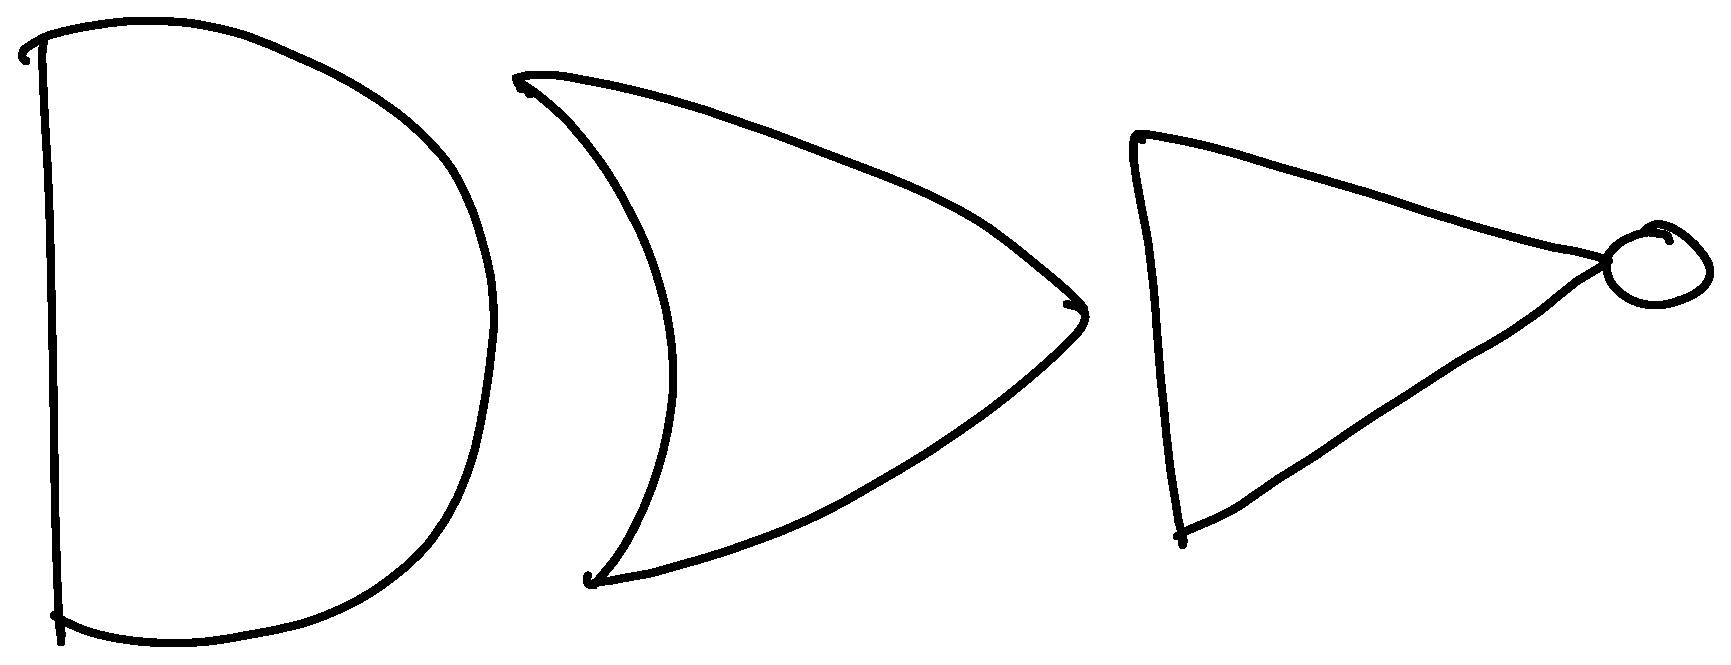
\includegraphics[width=1.0\hsize]{gates}
%\else 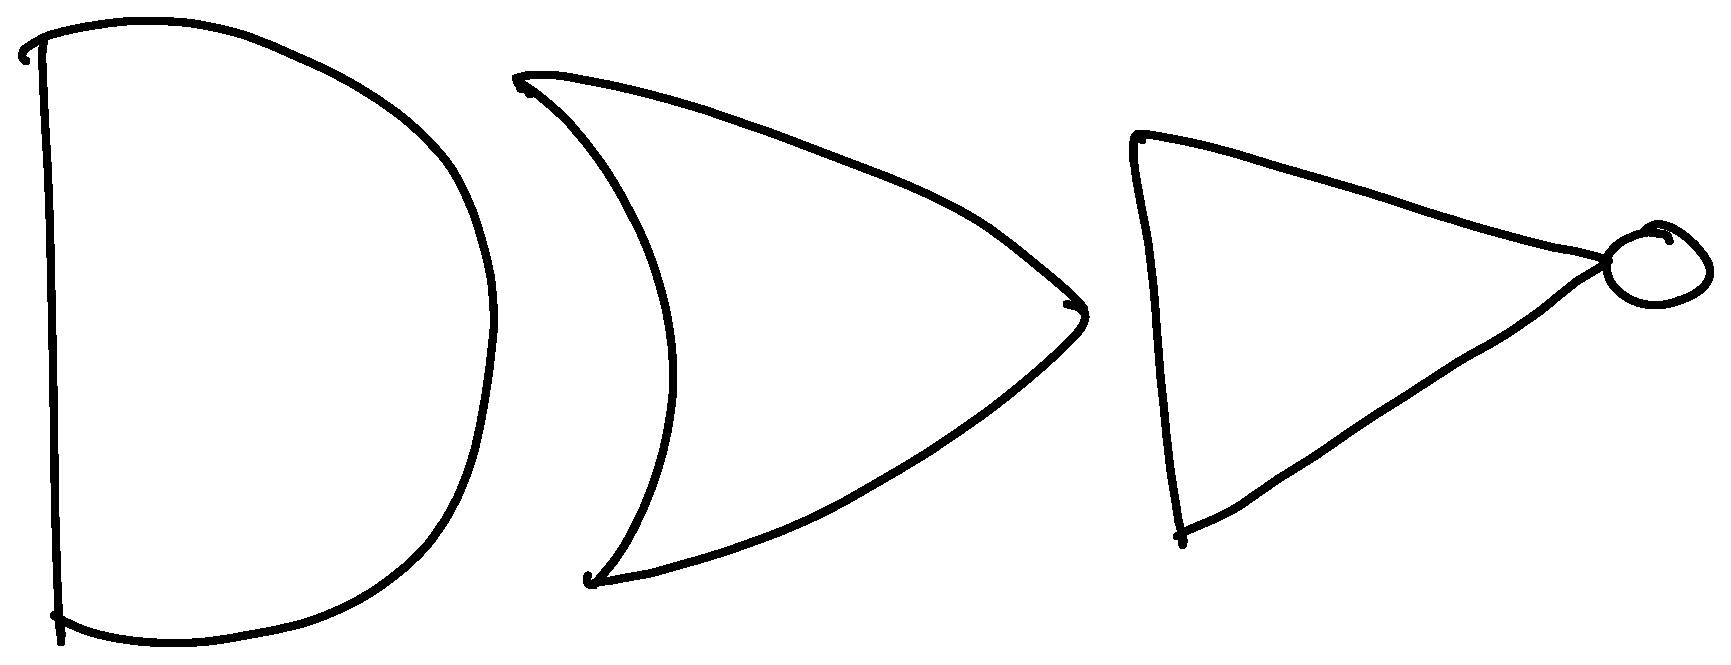
\includegraphics[width=1.0\hsize]{gates.eps} \fi
%\caption{The digital logic gate symbols used in this study. From the left: AND, OR, NOT.}
%\label{gatesFig}
%\end{figure}


\subsection{Data Sets}
\label{datasets}
We used two data sets for our experiments: a data set we collected
in the digital circuit domain, and the data set that was used in~\cite{schmieder09}
consisting of simple shapes (rectangles, lines, and ellipses), 
entity relationship diagrams, and process diagrams.  We collected
the first data set explicitly to examine the question of how 
task affects recognition accuracy.  We include the 
second data set for two reasons.  First, it provides 
confidence that the trends we observe are valid
and not a result of inadvertent bias in our collection process.  Second,
it contains a different set of shapes, allowing us to verify
these trends over a larger number of shapes.


\subsubsection{Dataset 1: Digital Circuit Diagrams}
We collected digital circuit diagram sketch data from 24 subjects, all
college students.  We call this dataset the Circuit Data.
We focus on digital logic diagrams because previous
work found that students tend to vary their drawing style in this
domain~\cite{alvarado07}, and recognizing the symbols in
this domain is particularly challenging because many symbols look
similar. The participants sketched freely on both Tablet PCs and Wacom 
tablets that used an inking pen on physical paper which was placed on top of 
the tablet; the data collection program performed no recognition.

We asked subjects to perform the three tasks described above: isolated
shape drawing (ISO), diagram copying (COPY), and diagram synthesis
(SYNTH).  The tasks were not necessarily performed in this order---we
balanced the task orders by having four 
students completed the tasks in each of the six order permutations.
In the ISO task we asked participants to draw ten isolated
instances of each single gate: AND, OR, and NOT, the most common gates
in digital circuit design.  In the COPY task, participants were asked
to copy two entire circuit diagrams (Figure~\ref{copyFig}).  In the
SYNTH task, participants were shown the following logical equations
(one at a time)
\[
Y1 = (\overline{(AB+C)}\oplus\overline{AC})+B+C \\
\]
\[
Y2 = (\overline{A}+BC)(A\overline{B}+AC+B)
\]
and told to create a circuit that satisfies each.  
Figure~\ref{synthFig} shows an example of one subject's
sketch for the first equation above.  
This task
simulates a ``real-world'' activity, as it is analogous to homework
problems students typically complete in a digital circuit design
class.  
For the copied and synthesized diagrams, we analyze only the AND,
OR and NOT gates because there were not enough of the other gates for
meaningful analysis.  

\begin{figure}
\mbox{ 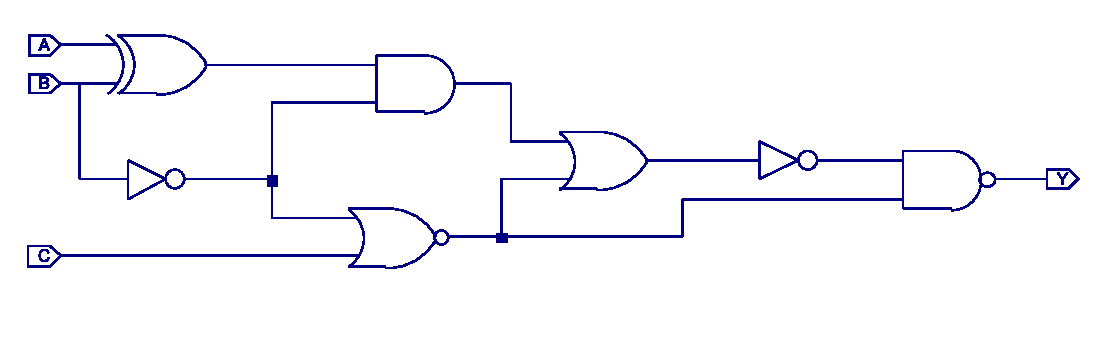
\includegraphics[width=1.0\hsize]{circuit_1.eps} }
\mbox{ 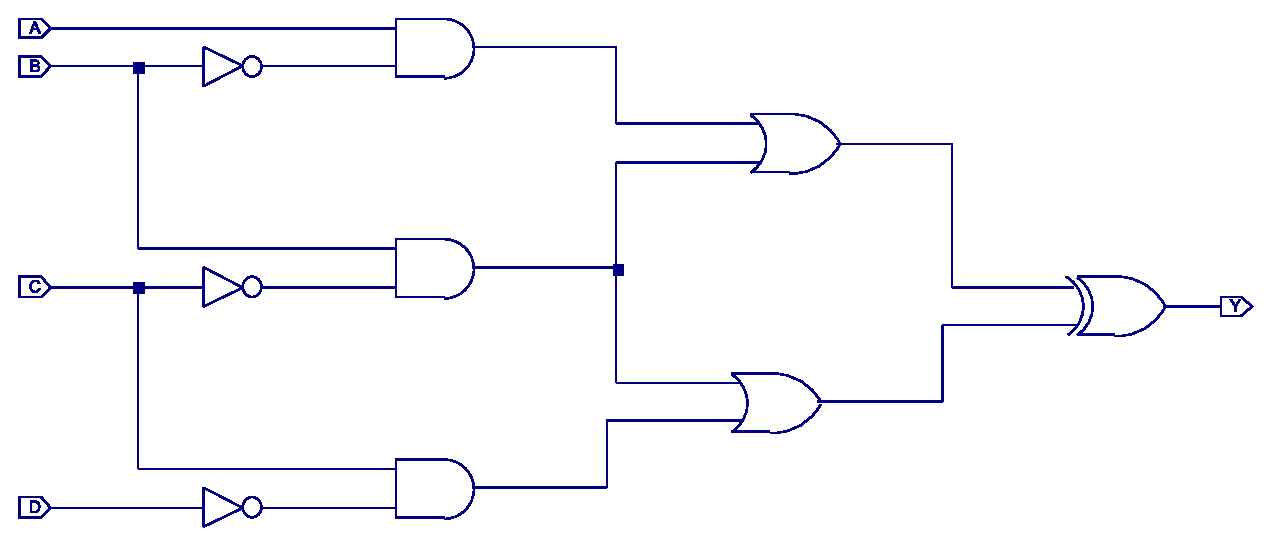
\includegraphics[width=1.0\hsize]{circuit_2.eps} }
\caption{The circuits participants copied in our study}
\label{copyFig}
\end{figure}

\begin{figure}
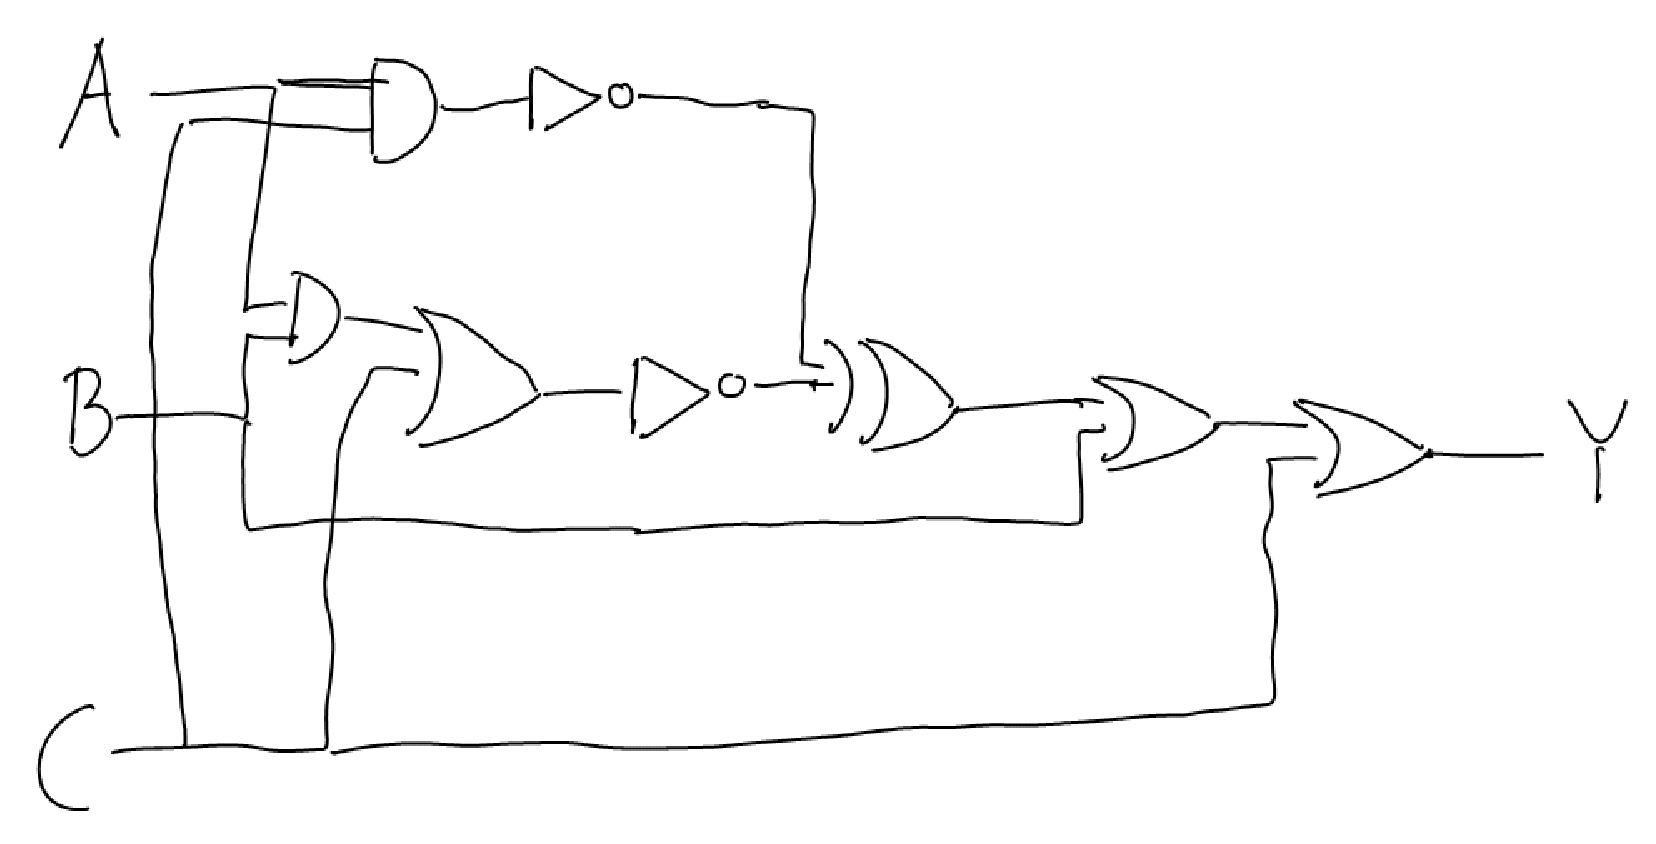
\includegraphics[width=1.0\hsize]{eqDrawing.eps}
\caption{One subject's sketch for the first synthesis equation}
\label{synthFig}
\end{figure}

\subsection{Dataset 2: Basic Shapes, Entity Relationship and Process Diagrams}
We also use the data from~\cite{schmieder09} to provide a wider base for our conclusions.
We call this dataset the Automatic Evaluation Data (after the title of~\cite{schmieder09}).
This data encompasses three tasks: isolated drawing of basic shapes (ISO),
drawing entity--relationship diagrams (ER), and drawing process diagrams (PROCESS).
The ISO task here is the same as it was above, but with different shapes which are
given below.
The ER and PROCESS tasks are both similar to our SYNTH task: users were asked 
to synthesize Entity-Relationship and Process diagrams.  Examples of these types of
diagrams are shown in Figures~\ref{fig:ER} and~\ref{fig:Process}.

The full Automatic Evaluation data set contains a fairly large body of shapes: 
circle, rectangle, diamond, line, arrow head, ellipse, and triangle.  
The authors of \cite{schmieder09} limited their experiments to 
ellipses, rectangles, and lines drawn with a single stroke because of the limitations 
of some of the recognizers they used.  In order to match their experiments,  
we also examined only ellipses, rectangles, and lines.  
However, because all of our recognizers are multi-stroke capable, we also included 
the multi-stroke rectangles.

\begin{figure}
\begin{center}
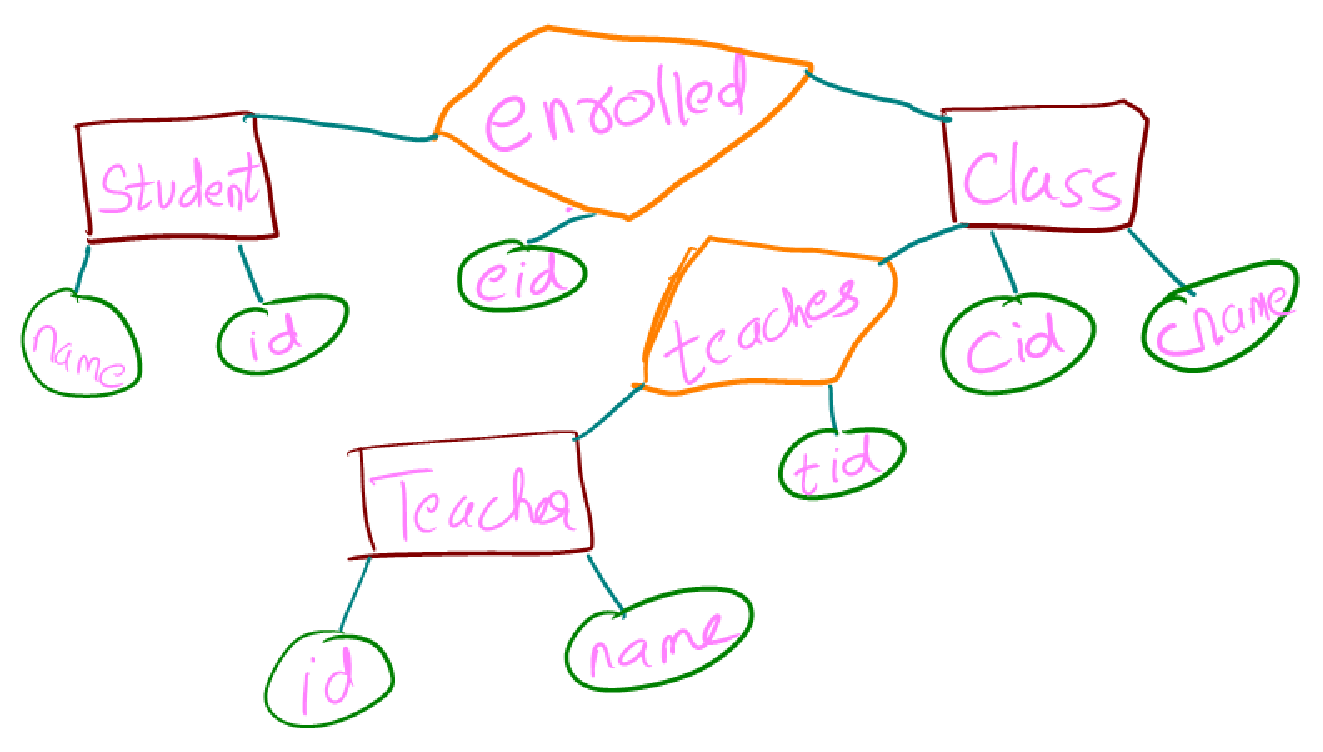
\includegraphics[width=.95\hsize]{ER.eps}
\end{center}
\caption{Example Entity-Relationship (ER) sketch.}
\label{fig:ER}
\end{figure}
\begin{figure}
\begin{center}
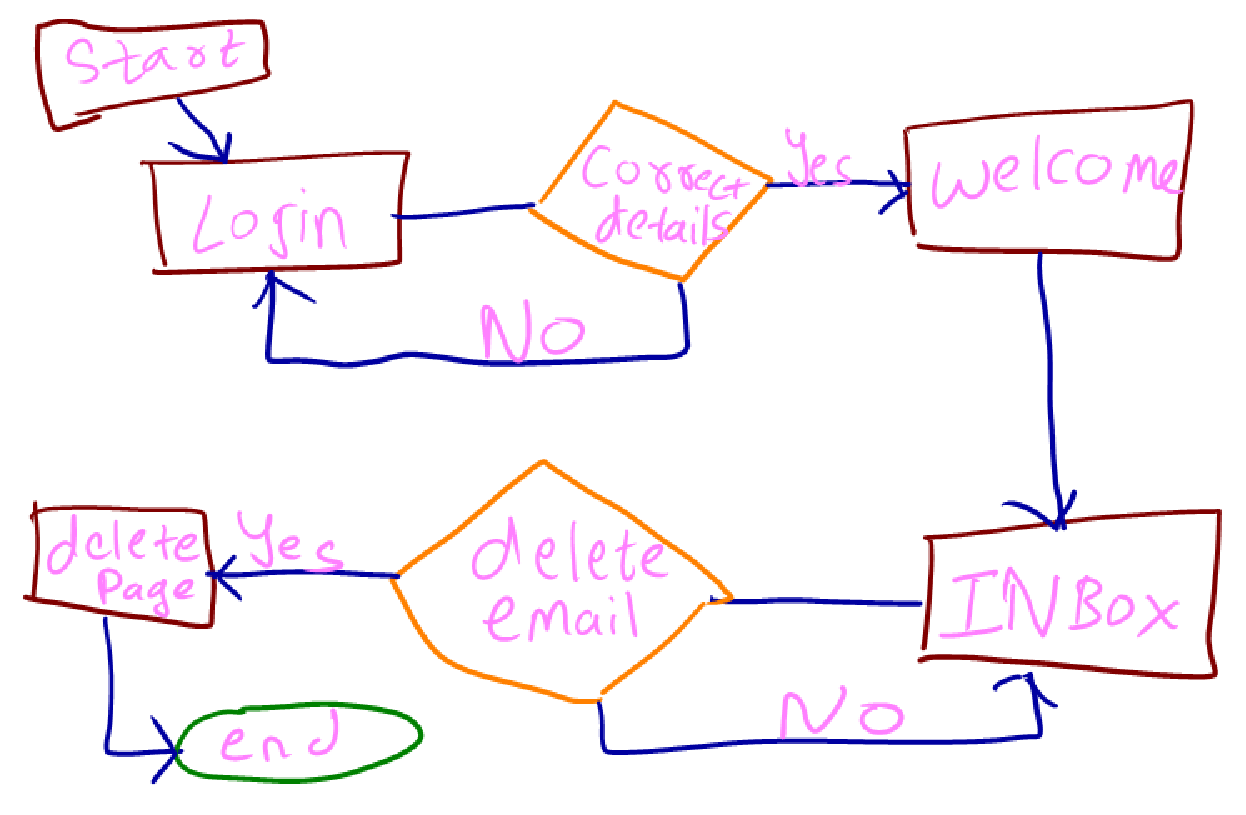
\includegraphics[width=.95\hsize]{Process.eps}
\end{center}
\caption{Example Process diagram sketch.}
\label{fig:Process}
\end{figure}

\section{Recognizers}
In our experiments, we use three distinct recognizers: two gesture
recognizers which are extensions of the \$1 recognizer~\cite{wobbrock07}, and an
existing Image-Based symbol recognizer~\cite{kara05}.
We created one extension of the \$1 recognizer, which we call
the ``multi-dollar'' recognizer, specifically for these experiments;
the authors of the original \$1 recognizer created the other extension, which they
call the ``\$N'' recognizer.  We chose to include
modified gesture recognizers because we wanted to test how sensitive
simple gesture recognition techniques are to drawing style.

\subsection{Multi-dollar recognizer}
We adapted the \$1 gesture recognizer to recognize multi-stroke symbols; 
we call this new recognizer multi-dollar.
The original single-stroke \$1 recognizer matches a stroke
to a template in four stages.  First, it resamples the
stroke to have the same number of equally-spaced points as the template.  
Second, it performs an initial rotation, using the
starting point of the stroke and its centroid to 
align the stroke with the template.
Third, it centers and scales the stroke to match the
center and scale of the template.  Finally, optimization
is used to refine the angular alignment between the
stroke and template. This process finds the 
angular alignment that results in the smallest path distance between
the stroke and the template. Path distance is defined as the sum of 
the distances between corresponding sample points. 

Our first modification was to the resampling step.  Rather than
resampling each stroke to a specific number of points, we
resample each \textit{shape} to a specific  number of points, 
regardless of how many strokes it contains (we use 48
points in our templates).  The number of sample points on a stroke
is proportional to the ratio of its
stroke length to the total length of the strokes in the shape, such
that the total number of points from all the strokes totals 48.  The first point 
of each stroke is always included as a sample point. 

The initial rotation, centering, and rescaling steps remain largely
unchanged. However, instead of centering on the centroid of one stroke, we use
the centroid of the whole symbol. Similarly, we resize the whole
symbol to a $64\times 64$ pixel bounding-box.

In the final step, the rotation search remains the same, but the
distance function used to guide the search is heavily modified.  
As in the original algorithm, we
require a one-to-one match between the points in the symbol
to be classified and the points in the template, but we can no longer use drawing
order to determine this match, as we want our
algorithm to be robust to variations in drawing order.  We instead 
minimize the sum of the distances between
each pair of matched points.  We have implemented two methods to perform this
minimization.

The above minimization problem is an instance of the assignment problem. Our two sets of points represent the vertices of a bipartite graph where the edge weights are the distances between the points.  We wish to assign each point in one set a match in the other set such that the sum of the edge weights is minimized.  One polynomial time solution to the assignment problem is the Hungarian algorithm~\cite{munkres57}.  We apply this algorithm to our problem as follows.
First, we calculate the distance from each point in the test shape to each point in the template; this initializes our weighted bipartite graph.  From here, it is a straightforward application of the Hungarian algorithm to find the lowest-cost matching.  We refer to this version of our multi-dollar recognizer as multi-dollar-HA (or MDHA). The Hungarian algorithm runs in O($N^3$) time, where $N$ is the number of points in the resampled shape. 

Another approach to the minimization problem is to approximate a solution using simulated 
annealing.  With this method, we also begin by calculating the distance from each point in the test 
shape to each point in the template.  Next, we create an initial search state using a greedy algorithm to 
match points in the test shape to the lowest-cost available points in the template.  New search states are 
generated by randomly selecting two points in the test shape and swapping their matches.  We refer to this 
version of our multi-dollar recognizer as multi-dollar-SA (or MDSA). The 
simulated annealing approach theoretically runs in O($N^2$) time because of the initial distance 
calculation. However, in our case, with a small $N$ and a large number of iterations, the actual run 
time increases linearly with $N$.

Before starting our main experiments, 
we ran a small set of experiments with both the Hungarian algorithm 
and simulated annealing versions of 
the multi-dollar recognizer to directly compare the two techniques.  
Using 48 points per shape, both algorithms take a comparable amount 
of time, but the Hungarian algorithm achieves a marginally better recognition accuracy.  As the number
of points per shape is increased, however, the Hungarian algorithm becomes untenably slow and the 
simulated annealing algorithm begins to close the performance gap.  In terms of code, simulated 
annealing is much easier to comprehend and implement.

More flexible methods of point-matching, such as Dynamic Time Warping
(DTW), have been applied to gesture
recognition~\cite{wobbrock07, kristensson04}. The main difference between these
methods and ours is that they allow
multiple points in one shape to be matched to a single point in the
other. As noted in~\cite{kristensson04}, flexible matching of points
introduces additional ambiguity between similar templates and degrades
the accuracy of the recognizer.

\subsection{\$N recognizer}
After we completed our multi-dollar recognizer, the authors of the original \$1
recognizer released (but have not yet published) their own 
multi-stroke extension of the \$1 recognizer called the \$N
recognizer\footnote{http://depts.washington.edu/aimgroup/proj/dollar/ndollar.html}.
Their approach is similar to ours, with two main differences.
First, instead of using a complex matching algorithm like ours, 
the \$N recognizer matches points temporally, just like the \$1 recognizer.
To guard against drawing style variation, the \$N recognizer searches over 
all stroke order and direction permutations.  A second important difference
between their method and ours is that they link multiple strokes together
before the resampling step.  This linking considers the ink that was drawn
``in the air'' from the end of one stroke to the beginning of the next.  These
virtual points then take away from the total number of points sampled from
the actual ink drawn (because the total number of points remains fixed). 
The authors discuss some of the known weaknesses of their algorithm\footnote{http://depts.washington.edu/aimgroup/proj/dollar/limits/}.

\subsection{Image-Based classifier}
We also used the Image-Based Trainable Symbol
Recognizer in \cite{kara05}.  The Image-Based recognizer,
like multi-dollar and \$N, is based on template matching.
Shapes are ``quantized'' into a $48\times 48$ pixel binary bitmap templates
and recorded in both cartesian and polar coordinates.  The polar version
of the template is used for angular alignment and elimination of unlikely definitions.
Once the optimal alignment of an unknown and definition has been computed
the cartesian version of the template is used for the final classification.
Classification relies on four image matching techniques whose
results are combined with a voting scheme. 
Because this algorithm was originally designed to recognize multi-stroke symbols,
it provides a nice contrast to the multi-dollar and \$N recognizers.
Furthermore, because the Image-Based recognizer is based on template matching,
it is very easy to add user-specific training examples.  Hence, it is especially
well suited to both aspects of our experiments.

% Rubine is being removed from the paper, right?
% Since we redid the tests and the test procedure, we don't really have any
% valid rubine results... --marty
%\subsection{Modified Rubine classifier}
%The Rubine classifier~\cite{rubine} is a standard and widely-used
%gesture classifier that works by extracting features from a
%single-stroke gesture and then training a linear classifier.  We used
%a simple approach to adapt the Rubine classifier to multi-stroke
%symbols: we simply join the strokes together in temporal order.  We
%then use the same features and the classification algorithm as in
%the original approach.  We expect that this adaptation will be highly
%sensitive to stroke order, and thus we expect the modified Rubine classifier to
%be the least robust of our three recognizers.

\section{Experiments and Results}
The primary goal of our experiments was to determine how potential drawing-style 
variations between tasks affects recognition accuracy.  We used two approaches to
address this goal.  First, we compared stroke properties of shapes
drawn under different task conditions to get a sense for how much drawing
style actually varies between tasks.  Second, we trained and tested our recognizers
on data collected during different drawing tasks and measured variations in
recognition accuracy.  

In addition to this primary goal, we had two secondary goals.
First, we wanted to
determine how much impact user-specific training data has on recognition
accuracy.  Second, we wanted to directly compare the performance of our recognizers
on the free-sketch data we are interested in ultimately recognizing.

\subsection{Drawing Style Across Tasks}
\label{style}

To provide one measure of the effect of task on drawing style, we
examined how stroke order varies with task for our digital circuit
data. By stroke order, we mean the number of strokes used to draw a
shape, and the order in which they occur. For example, AND gates are
often drawn with either a single stroke, or with two strokes ---  one
representing the back of the gate, the other representing the
remainder of the gate. The strokes in the two-stroke version of the
gate can be drawn in either order.

To begin, we examined drawing-order consistency within a task. For a
given task, many users either had a single dominant stroke order or
had a nearly equal preference for two drawing orders. More precisely,
we consider a user to have a {\em dominant} style if at least 80\% of
shapes were drawn with the same stroke order. Likewise, we consider a
user to have a {\em split} style if two drawing orders account for at
least 80\% of the shapes, and the frequency of those orders differs by
no more than 20 percentage points (e.g., one order was used 50\% of
the time and another was used 45\% of the time). 


Table \ref{tab:dominant} summarizes the results of the within-task
consistency analysis.  Most of the 24 subjects who provided digital
circuit data had a dominant style for AND gates for each of the three
tasks: ISO, COPY, and SYNTH.  (While style was consistent within a
task, it may still vary between tasks; this is considered below.) For
OR gates, half of the subjects had a dominant drawing style for all
tasks, while between 21\% and 38\% had a split style, depending on the
task.  The results for NOT gates for the ISO and COPY tasks are
similar to those for OR gates. For the SYNTH task, however, many
subjects drew an insufficient number of NOT gates (instead preferring
to add NOTBUBBLEs to gates) to enable meaningful analysis. We excluded
from the analysis any subject who did not draw at least 5 examples of a
particular gate. For the SYNTH task, only seven subjects drew an
adequate number of NOT gates. 

As a remedy, we combined the COPY and SYNTH data to produce an
artificial COPSYN task, representing drawing shapes in the context of
a larger drawing task. For the AND and OR gates, two fewer subjects
had a dominant style for the COPSYN task than for either the COPY or
SYNTH tasks. This suggests that some users had dominant styles for one
or both of the COPY and SYNTH tasks, but their preferences  varied
between these tasks.  For NOT gates, 39\% of the 23 users who had adequate
data had a dominant style for the COPSYN task, while 26\% had a split
style.


\begin{table}
\centerline{\begin{tabular}{|c|c|cccc|}
\hline
Gate & Mode & ISO & COPY & SYNTH & COPSYN \\ \hline
\multirow{2}{*}{AND} & Dominant & 24 & 21 & 21 & 19 \\ %\cline{2-6}
                     & Split    & 0  & 0  & 0  & 1 \\ \hline
\multirow{2}{*}{OR}  & Dominant & 13 & 12 & 12 & 10 \\ %\cline{2-6}
                     & Split    & 9  & 7  & 5  & 5 \\ \hline
\multirow{2}{*}{NOT} & Dominant & 13 & 11 & 5* & 9** \\ %\cline{2-6}
                     & Split    & 8  & 6  & 0* & 6** \\ \hline
\end{tabular}}
\caption{Number of users, out of 24 total, with a Dominant or Split drawing style. 
*Only seven users had sufficient data. **Only 23 users had sufficient data.}
\label{tab:dominant}
\end{table}

Table \ref{tab:dominant} demonstrates that most users have either a
dominant or split style within a task. An equally important issue is
consistency across tasks. Table \ref{tab:persistence} shows the number
of users who maintained a consistent style between the ISO task and
each of the other tasks. For AND gates, between 18 and 21 users
maintained a consistent style across each of the pairs of tasks
(i.e., they had the same preferred style for both). For OR gates, there was
less consistency across tasks. For example, only nine users had the
same style (seven dominant styles and two split styles) for both
the COPY and SYNTH tasks. For NOT gates, there appears to be little
consistency, but again, in many cases too few gates were drawn to
enable meaningful analysis.


As another measure of across-task consistency, we also compute an aggregate
measure of the variation of stroke-order frequencies between tasks. We define
the distribution difference as:


\begin{equation}
\delta = \frac{1}{2}\displaystyle\sum_{i=1}^{N} |SO_{i}(Task_{a}) - SO_{i}(Task_{b})|
\label{eqn:delta}
\end{equation} 

\noindent
where $N$ is the number of unique stroke orderings, and $SO_i$ is the
fraction of shapes drawn with Stroke Order $i$. For example, if the
ISO task comprises 80\% stroke order A and 20\% stroke order B, while
the COPY task comprises 90\% A and 10\% B, the distribution difference
would be 10\%.  The $1/2$ normalization factor essentially characterizes
this difference in terms of each distribution's total deviation from the
the average of the two.

Table \ref{tab:deltas} contains the results of the distribution
difference analysis. For AND gates, the difference ranges from 9\% to
16\%. For OR gates, there is more variation, ranging from 19\% to
25\%. For NOT gates, the variation is 35\% to 37\% for cases in which
there is adequate data to perform meaningful analysis.

These analyses suggest that while stroke order remains moderately
consistent both within and across tasks, variation in stroke order must
be considered when training a recognizer. A key question is, how many
stroke orders should be considered? Table \ref{tab:toporders} lists
the average percentage of shapes drawn by each user with the single
most popular stroke order, the two most popular stroke orders, and the
three most popular stroke orders. For all tasks, the top three stroke
orders accounted for at least 92\% of the shapes drawn.


\begin{table}
\centerline{\begin{tabular}{|c|c|cccc|}
\hline
Gate & Mode & I-C & I-S & C-S & I-CS \\ \hline
\multirow{2}{*}{AND} & Dominant & 21 & 20 & 18 & 19 \\ %\cline{2-6}
                     & Split    & 0  & 0  & 0  & 0  \\ \hline
\multirow{2}{*}{OR}  & Dominant & 12 & 9  & 7  & 10 \\ %\cline{2-6}
                     & Split    & 4  & 4  & 2  & 5  \\ \hline
\multirow{2}{*}{NOT} & Dominant & 8  & 3* & 3* & 6**\\ %\cline{2-6}
                     & Split    & 3  & 0* & 0* & 3**\\ \hline
\end{tabular}}
\caption{Persistence of stroke orders across tasks. 
I=ISO, C=COPY, S=SYNTH, CS=COPSYN.
*Only seven users had sufficient data. **Only 23 users had sufficient data.}
\label{tab:persistence}
\end{table}

\begin{table}
\centerline{\begin{tabular}{|c|cccc|}
\hline
Gate & I-C & I-S & C-S & I-CS \\ \hline
AND & 9\%  & 15\% & 16\% & 12\% \\ %\hline
OR  & 19\% & 24\% & 25\% & 20\% \\ %\hline
NOT & 35\% & -  & -  & 37\% \\ \hline
\end{tabular}}
\caption{Differences in between-task stroke-order frequencies, averaged
across users. I=ISO, C=COPY, S=SYNTH, CS=COPSYN.
'-' = insufficient data.}
\label{tab:deltas}
\end{table}

\begin{table}
\centerline{\begin{tabular}{|c|c|ccc|}
\hline
Gate & Mode & ISO & COPY & SYNTH \\ \hline
\multirow{3}{*}{AND} & Top 1 & 95 & 91 & 85 \\
                     & Top 2 & 98 & 98 & 94 \\
					 & Top 3 & 99 & 99 & 99 \\ \hline
\multirow{3}{*}{OR}  & Top 1 & 74 & 68 & 70 \\
                     & Top 2 & 95 & 85 & 88 \\
					 & Top 3 & 98 & 95 & 93 \\ \hline
\multirow{3}{*}{NOT} & Top 1 & 76 & 65 & 72 \\
                     & Top 2 & 95 & 84 & 94 \\
					 & Top 3 & 97 & 92 & 96 \\ \hline
\end{tabular}}
\caption{Average percentage of shapes drawn by each user with the (1) Single most popular 
stroke order, (2) two most popular stroke orders, and (3) three most popular stroke orders.}
\label{tab:toporders}
\end{table}

\subsection{Recognition Experiments}
\label{experimentOverview}

In the previous section we showed that there are indeed
differences in drawing styles across tasks, between users
and between shapes for a single task for a single user.
In the next three sections, we present quantitative experiments
examining the effect these variations have on recognition
accuracy.  In these experiments, we vary three independent
variables: drawing task, the amount of user-specific training data,
and the recognizer.  As described in Section~\ref{datasets}, the digital
circuit data includes three tasks: ISO, COPY, and SYNTH. Likewise,
the Automatic Evaluation data also includes three tasks: ISO, ER,
and PROCESS. We consider four recognizers: \$N, multi-dollar-HA (MDHA),
multi-dollar-SA (MDSA), and Image-Based (Img).

To examine the effects of user-specific training data, we consider
three conditions: user independent --- no user-specific data, user
semi-dependent --- a mix of user-specific and user-independent data,
and user-dependent --- user-specific data only.  For the
user-independent condition, we first randomly split the users
into two equal partitions, one for
testing and one for training.  Note that this split ensures that
no user-specific data will be used for any test, since the testing users
are distinct from the users from which we draw the training data.  
We randomly select five examples of
each shape from the training partition for use in training the
recognizers.    We call this condition the GlobalSet, and it simulates
the experience of a ``factory-trained'' recognizer that cannot be
customized for a particular user, which is the normal situation for
most sketch recognition systems.  

We chose five examples because all of the recognizers we use
are instance-based techniques, recognition cost increases with the
number of training examples.   Five examples provided an acceptable
trade-off between running time and accuracy; we found that accuracy increased
only slightly, or not at all in some cases, with more examples. 

For the user semi-dependent condition, we again set aside 50\% of the
users for training, but this time we select only two examples of each
shape from this set.  Then, we create a separate classifier for each
user by randomly selecting three examples from their own data, adding
those examples to the two chosen from the training users, and removing
these examples from their test set (i.e., we never trained and tested
on the same examples).  We call this condition the ComboSet, and
it simulates the experience of a factory-trained recognizer that has
been tuned by the user by providing examples.

For the user dependent condition, we simply randomly select five
examples of each shape from each user's data (and remove those
examples from the test set) to train a single recognizer for each
user.  We call this condition the UserSet, and it simulates a
recognizer trained only on examples provided by the user. 
When there are five or fewer examples of a given shape for training 
we cannot train the UserSet completely and instead use $n$-1 examples 
where $n$ is the number of symbols for that user.




\subsubsection{The Effect of Task on Recognition Accuracy}
\label{taskExperiment}
\begin{table*}
\centerline{\begin{tabular}{|l|cccc|cccc|cccc|}
\hline
 Activity & \multicolumn{4}{|c|}{GlobalSet} & \multicolumn{4}{|c|}{ComboSet} & \multicolumn{4}{|c|}{UserSet} \\
 (train-test) & \$N & MDSA & MDHA & Img & \$N & MDSA & MDHA & Img & \$N & MDSA & MDHA & Img \\
\hline
ISO-ISO & 84.1 & 	86.2 & 	89.1 & 	83.5 & 	94.6 & 	94.5 & 	96.6 & 	94.6 & 	93.1 & 	94.6 & 	96.4 & 	93.5 \\
COPY-ISO & 82.0 & 	87.4 & 	89.5 & 	81.0 & 	89.5 & 	92.0 & 	94.1 & 	89.0 & 	82.9 & 	90.1 & 	92.3 & 	83.9 \\
SYNTH-ISO & 79.4 & 	84.5 & 	88.0 & 	82.1 & 	87.2 & 	89.8 & 	93.1 & 	88.8 & 	72.1 & 	77.1 & 	80.1 & 	76.8 \\
\hline
ISO-COPY & 83.9 & 	88.3 & 	90.5 & 	87.0 & 	88.4 & 	92.3 & 	95.0 & 	93.0 & 	83.1 & 	89.5 & 	93.4 & 	88.4 \\
COPY-COPY & 82.4 & 	89.7 & 	91.2 & 	85.7 & 	91.5 & 	94.8 & 	96.5 & 	96.1 & 	90.2 & 	94.4 & 	96.6 & 	95.3 \\
SYNTH-COPY & 79.0 & 	86.4 & 	90.5 & 	86.6 & 	87.3 & 	91.8 & 	95.1 & 	91.7 & 	71.7 & 	76.1 & 	80.4 & 	77.2 \\
\hline
ISO-SYNTH & 78.5 & 	79.3 & 	84.1 & 	81.1 & 	84.8 & 	84.3 & 	88.4 & 	88.5 & 	79.6 & 	82.7 & 	86.6 & 	84.0 \\
COPY-SYNTH & 77.7 & 	82.0 & 	84.6 & 	79.4 & 	85.5 & 	86.4 & 	88.2 & 	86.8 & 	82.0 & 	84.4 & 	87.5 & 	81.9 \\
SYNTH-SYNTH  & 73.1 & 	78.6 & 	83.0 & 	81.9 & 	84.5 & 	90.0 & 	93.7 & 	93.4 & 	83.8 & 	90.7 & 	94.3 & 	88.6 \\
\hline
\end{tabular}}
\caption{Recognition accuracy on the circuit data for all three recognizers, in percent.}
\label{tab:allResults}
\end{table*}

\begin{table*}
\centerline{\begin{tabular}{|l|cccc|cccc|cccc|}
\hline
 Activity & \multicolumn{4}{|c|}{GlobalSet} & \multicolumn{4}{|c|}{ComboSet} & \multicolumn{4}{|c|}{UserSet} \\
 (train-test) & \$N & MDSA & MDHA & Img & \$N & MDSA & MDHA & Img & \$N & MDSA & MDHA & Img \\
\hline
ISO-ISO & 79.3 & 	83.4 & 	85.3 & 	85.0 & 	90.8 & 	94.6 & 	95.0 & 	93.1 & 	89.3 & 	91.1 & 	93.1 & 	90.8 \\
ER-ISO & 81.5 & 	81.0 & 	85.8 & 	79.4 & 	84.5 & 	83.1 & 	89.2 & 	82.5 & 	72.2 & 	73.6 & 	79.7 & 	69.5 \\
PROCESS-ISO &75.8 & 	80.2 & 	84.9 & 	83.4 & 	79.3 & 	82.0 & 	87.2 & 	85.5 & 	64.3 & 	68.6 & 	74.2 & 	65.0 \\ 
\hline
ISO-ER & 73.6 & 	86.8 & 	88.9 & 	87.5 & 	79.8 & 	91.3 & 	92.6 & 	89.0 & 	73.6 & 	77.4 & 	82.6 & 	81.0\\ 
ER-ER & 84.2 & 	95.6 & 	92.2 & 	89.6 & 	90.1 & 	97.9 & 	97.1 & 	95.8 & 	83.1 & 	87.7 & 	90.3 & 	90.0 \\
PROCESS-ER & 76.2 & 	94.3 & 	95.5 & 	83.2 & 	84.8 & 	96.1 & 	96.8 & 	86.5 & 	64.2 & 	72.6 & 	75.7 & 	65.8 \\
\hline
ISO-PROCESS & 79.4 & 	80.8 & 	86.0 & 	75.2 & 	83.9 & 	84.9 & 	88.7 & 	77.0 & 	76.1 & 	69.7 & 	78.5 & 	70.7 \\
ER-PROCESS & 83.0 & 	88.5 & 	89.2 & 	83.6 & 	86.2 & 	91.6 & 	92.2 & 	86.7 & 	75.5 & 	75.5 & 	80.2 & 	72.7 \\
PROCESS-PROCESS & 81.4 & 	84.1 & 	88.6 & 	81.7 & 	92.6 & 	89.3 & 	93.0 & 	86.7 & 	90.5 & 	83.1 & 	88.1 & 	86.8 \\
\hline
\end{tabular}}
\caption{Recognition accuracy on the Automatic Evaluation data for all three recognizers, in percent.}
\label{tab:allResults2}
\end{table*}

\begin{figure*}[p]
\begin{center}
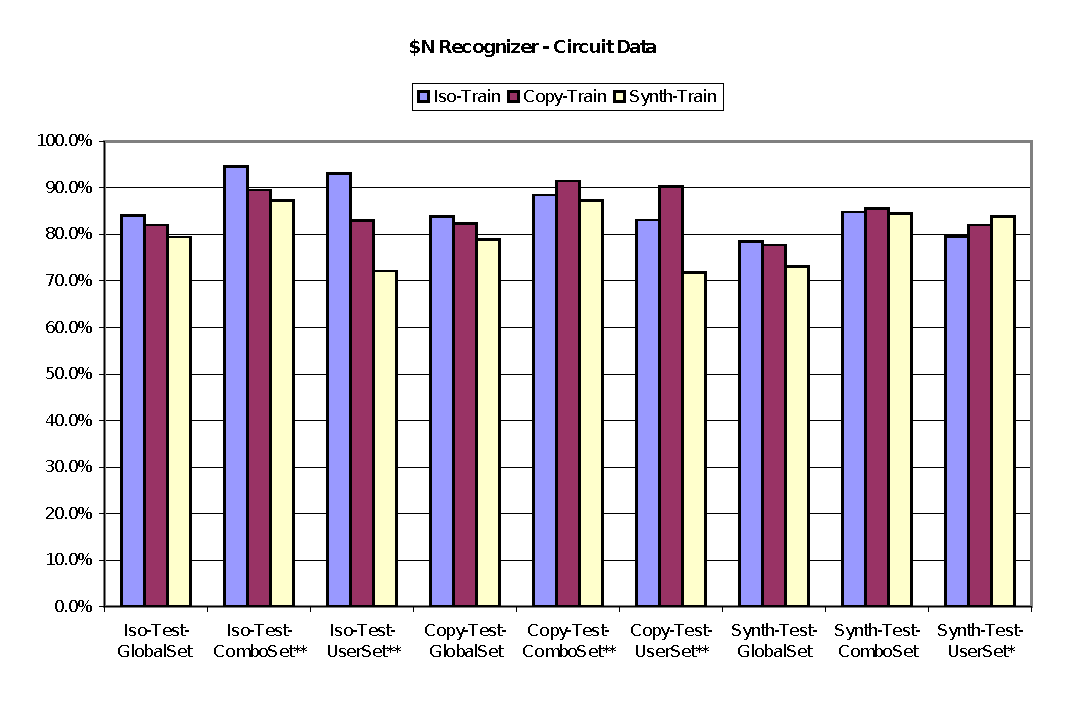
\includegraphics[width=.9\hsize]{NDollarCircuitChart.eps}
\end{center}
\caption{Recognition accuracy for the \$N with different training and testing sets. }
\label{NDollarCircuit}
\end{figure*}

\begin{figure*}[p]
\begin{center}
\includegraphics[width=.9\hsize]{MultiDollarSACircuitChart.eps}
\end{center}
\caption{Recognition accuracy for the MDSA with different training and testing sets. }
\label{MultiDollarSACiruit}
\end{figure*}

\begin{figure*}[p]
\begin{center}
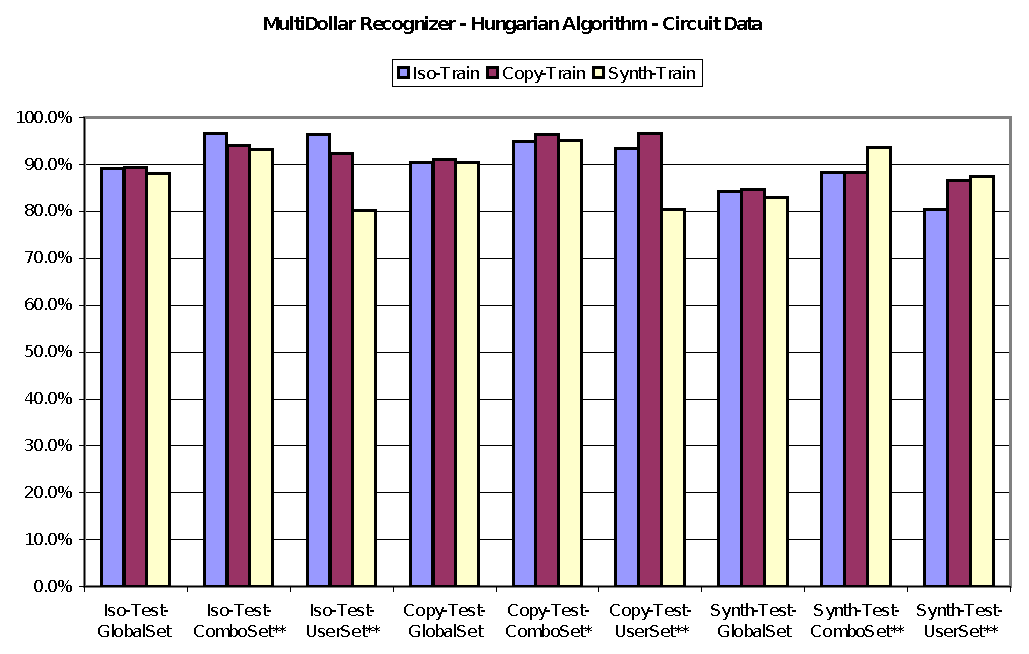
\includegraphics[width=.9\hsize]{MultiDollarHACircuitChart.eps}
\end{center}
\caption{Recognition accuracy for the MDHA with different training and testing sets. }
\label{MultiDollarHACiruit}
\end{figure*}

\begin{figure*}[p]
\begin{center}
\includegraphics[width=.9\hsize]{ImageRecoCircuitChart.eps}
\end{center}
\caption{Recognition accuracy for the Image-Based with different training and testing sets. }
\label{ImageRecoCircuit}
\end{figure*}

\begin{figure*}[p]
\begin{center}
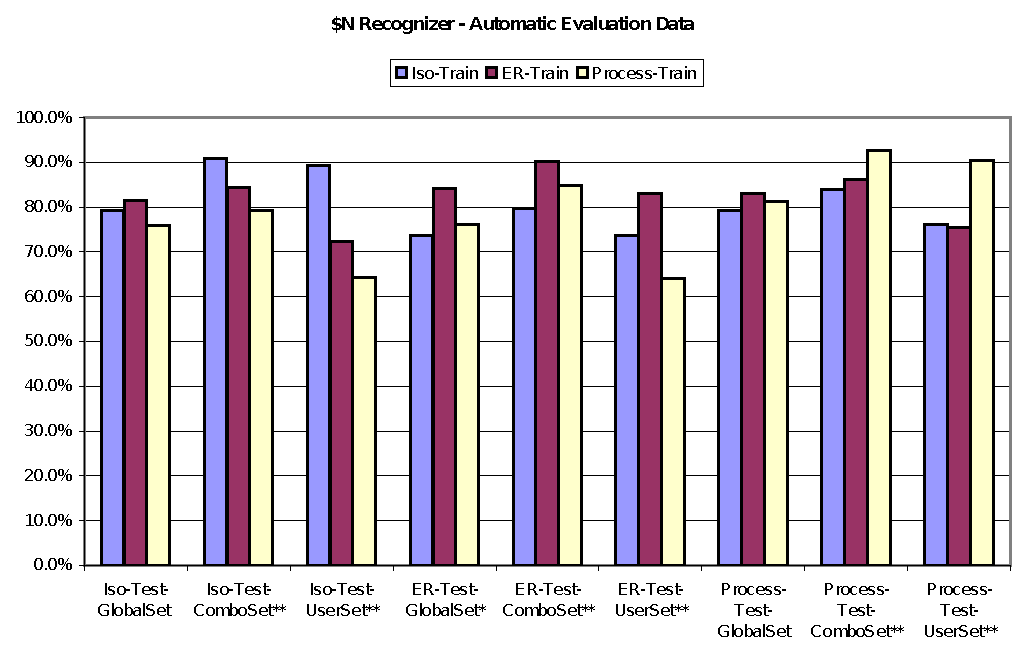
\includegraphics[width=.9\hsize]{NDollarAutoChart.eps}
\end{center}
\caption{Recognition accuracy for the \$N with different training and testing sets. }
\label{NDollarAuto}
\end{figure*}

\begin{figure*}[p]
\begin{center}
\includegraphics[width=.9\hsize]{MultiDollarSAAutoChart.eps}
\end{center}
\caption{Recognition accuracy for the MDSA with different training and testing sets. }
\label{MultiDollarSAAuto}
\end{figure*}

\begin{figure*}[p]
\begin{center}
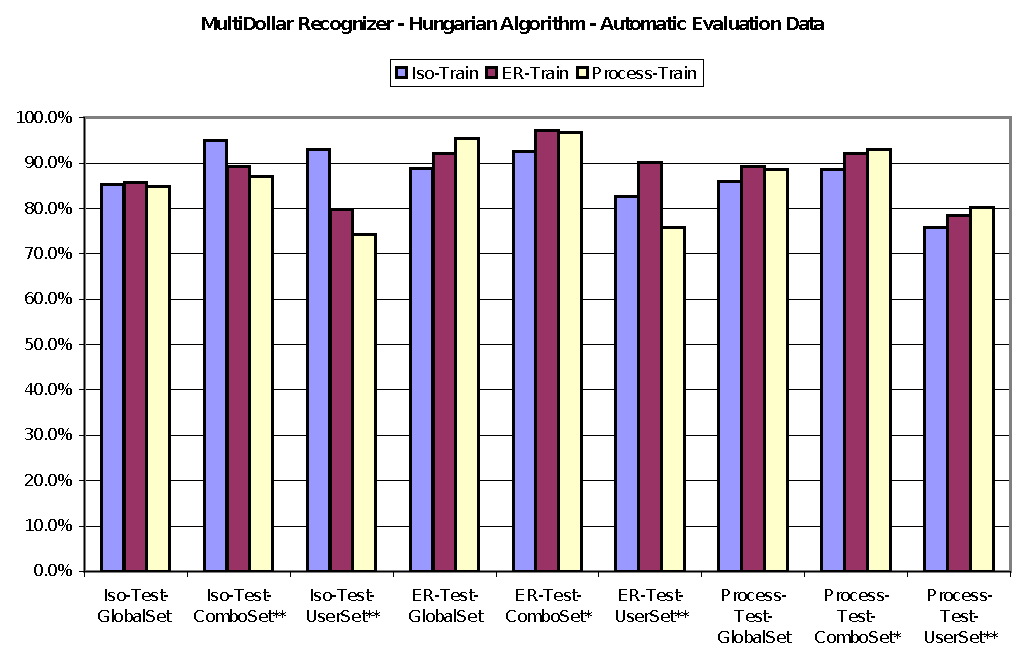
\includegraphics[width=.9\hsize]{MultiDollarHAAutoChart.eps}
\end{center}
\caption{Recognition accuracy for the MDHA with different training and testing sets. }
\label{MultiDollarHAAuto}
\end{figure*}

\begin{figure*}
\begin{center}
\includegraphics[width=.9\hsize]{ImageRecoAutoChart.eps}
\end{center}
\caption{Recognition accuracy for the Image-Based with different training and testing sets. }
\label{ImgRecoAuto}
\end{figure*}

In this section we examine the effect of task on recognition accuracy.
We consider this question in the context of the other two variables: recognizer
and amount of user-specific training data.

To examine these questions, we trained nine different versions of each
recognizer: one for each possible combination of the three training
tasks and the three levels of user-specific training data.  We then
tested each recognizer using data from all three tasks, resulting in a
total of 27 training-testing combinations for each recognizer.  For
example, the ISO / GlobalSet trained Image-Based recognizer was tested
on data from the ISO, COPY, and SYNTH tasks (for convenience, we refer
to these training-testing combinations as ISO-ISO, ISO-COPY, and
ISO-SYNTH). Note that this analysis was performed for both the Digital
Circuit and the Automatic Evaluation data sets. 

To generate more stable results, we ran 25 trials of the experiment.
The recognition accuracies we present are averages over all 25 runs.
However, the repeated measures ANOVA design used in the 
statistical analysis considers each run as a separate, independent measurement.
Within each trial, we first generated sets of training data that were used for 
all conditions and all recognizers.  We ensured three conditions:
training symbols were never used for testing, all four recognizers
were trained on the same shapes, and the same training data was always
used for a particular training condition (e.g. the ISO-ISO, ISO-COPY, ISO-SYNTH
tests were all performed using recognizers trained on the same ISO shapes).
This guarantees that we can directly compare the results from the different
conditions and recognizers.

%To generate more stable results, we ran 25 trials for each of the 27
%different training--testing combinations and averaged the results.  
%Within a single trial, we used consistent training and testing data across the various
%combinations of training and testing conditions. In particular, for
%each trial, we randomly partitioned the users into training/testing
%sets, as described above, and randomly selected the training and
%testing examples using the appropriate method.  We then trained each
%recognizer and ran each test using the same testing and training data across all
%training--testing combinations, as appropriate.  For example, in each
%trial there was a single GlobalSet for each task, which was used to
%train all recognizers for the GlobalSet condition for that task.
%Using consistent training and testing data ensures that results from
%the recognizers under different conditions are directly comparable.


%this is averaged over the 25 trials, right?
Tables~\ref{tab:allResults} and~\ref{tab:allResults2} present
 the average classification
accuracy for all combinations averaged over the 25 trials for the circuit
data and the Automatic Evaluation data, respectively.  
Figures~\ref{NDollarCircuit}--\ref{ImgRecoAuto} show these same results graphically.

%\note{what is a cluster? clusters of bars?}
%statistically significant or practically? 
%where is the anova and Bonferroni post-hoc results ? What do they mean?
In this section, we are interested in the individual clusters of bars in each 
graph.  Each of these clusters represents a single testing task for a single recognizer, 
with one bar for each of the training tasks.  

In this section we refer to statistically significant results as significant, however they 
may not necessarily result in a large difference in accuracy.

In many cases, it appears that
training and testing on data from the same task \emph{does} in fact improve
recognition accuracy over training on data from either of the other two tasks.
To test the statistical significance of these differences, we performed a repeated-measures
ANOVA on the data behind each of the clusters in Figures~\ref{NDollarCircuit}--\ref{ImgRecoAuto}.
We then performed a Bonferroni post hoc analysis to determine
which tasks led to significantly different recognition results.
We indicate the results of this analysis in the labels on the graphs.  
In Figures~\ref{NDollarCircuit}--\ref{ImgRecoAuto},
labels marked with a (*) indicate that training with task-specific data significantly
improved accuracy over exactly one of the other two tasks, while labels
marked with a (**) indicate that training with task-specific data significantly
improves accuracy over both other tasks (p $<$ 0.05).  For example, in Figure~\ref{MultiDollarHAAuto},
the leftmost cluster of bars shows that 
when testing on ISO data, there is no significant difference in the performance 
of the multi-dollar HA algorithm when it is trained on user-independent (GlobalSet)
data from the three different tasks.  For the ER task using user semi-dependent (ComboSet) data, 
training on data from the ER task produces significantly better recognition results than
training on data from the ISO task.  For the ER task using user-dependent (UserSet) data,
training on data from the ER task produces significantly better recognition results
than training on data from either the ISO or the PROCESS tasks. 

%\note{Our results show that whether or not task affects recognition accuracy depends
%on the amount of user-specific training data used to train the recognizer. Does this scale with
%amount: effect is greater for ComboSet than GlobalSet, and effect is greater for UserSet
%than ComboSet?}

In most cases, training on task-specific data does
significantly improve recognition accuracy. The exception is when the
training data includes no user-specific data. For the circuit data,
for instance, training on task-specific data produced no significant
increase in accuracy for the GlobalSet training condition --- there
are no asterisks following ``GlobalSet'' in
Figures~\ref{NDollarCircuit}--\ref{ImageRecoCircuit}.  For the
Automatic Evaluation data, there were only a few cases in which
training on task-specific data produced a significant increase in
accuracy for the GlobalSet training condition (ER-Test with the \$N
and multi-dollar-SA recognizers and PROCESS-test with the Image-Based
recognizer). Note that these differences are small compared to
the differences using the Combo and User sets.  Furthermore,
in most of these cases, training on task specific data significantly
improved accuracy over only one of the other two task conditions (i.e. *
instead of **). 
%how do we define slight?  % are these all of the cases? 


Tables~\ref{tab:allResults}
and~\ref{tab:allResults2} and Figures~\ref{NDollarCircuit}--\ref{ImgRecoAuto}
also show that as we increase the amount of user-specific training data, 
recognizers become more sensitive to task.  In general, the task specific bar
in the UserSet clusters tends to stand out more from the other two bars than it 
does in the ComboSet and GlobalSet clusters.  

Table~\ref{tab:allResults2} and Figures~\ref{NDollarAuto}--\ref{ImgRecoAuto} also 
show that domain in addition to task affects recognition accuracy.  Both ER
and PROCESS are synthesis tasks.  Yet in many cases, a recognizer trained on ER
data significantly out-performs a recognizer trained on PROCESS data when applied
to recognize ER diagrams, and vice-versa.


\subsubsection{The Effect of User-Specific Data on Recognition}
\label{userExperiment}
It is clear from Figures~\ref{NDollarAuto}--\ref{ImgRecoAuto} that the 
amount of user-specific training data affects overall recognition accuracy, 
as well influencing how much task affects accuracy.  In this section, we specifically 
explore how recognition performance changes as
we increased the amount of user-specific training data used to train
the recognizer.

% which user-data experiment?

In this section we focus on the ISO-SYNTH, ISO-ER and ISO-PROCESS training-testing data specifically.  
We chose these training-testing combinations because they simulates a real-world 
situation.  We imagine that a user has acquired a ``factory-trained'' recognition system (such
as the system produced with the GlobalSet training method above), and now has the
option of training the system by drawing isolated shapes.  We want to
know how much (if at all) this user-specific data will improve
classification accuracy.

With the data from the previous experiment, we have enough information to answer this question.  For
each of the 25 runs and each of the four recognizers, we calculated the average performance 
over all testing users for the GlobalSet, UserSet, and ComboSet variants for the ISO-SYNTH condition.  
We also performed this experiment with the Automatic Evaluation data, instead using an average 
of both the ISO-ER and ISO-PROCESS conditions.  
\begin{table}
\centerline{\begin{tabular}{|c|l|l|}
\hline
Recognizer & Comparison & P - Bonf. \\
\hline
 & ComboSet and GlobalSet & $\mathbf{<0.001}$ \\
multi-dollar HA & ComboSet and UserSet &$\mathbf{<0.001}$ \\
 & UserSet and GlobalSet & \textbf{0.019} \\
 \hline
 & ComboSet and GlobalSet & $\mathbf{<0.001}$ \\
multi-dollar SA & ComboSet and UserSet & \textbf{0.012} \\
 & UserSet and GlobalSet & $\mathbf{<0.001}$ \\
 \hline
 & ComboSet and GlobalSet & $\mathbf{<0.001}$ \\
\$N & ComboSet and UserSet & $\mathbf{<0.001}$ \\
 & UserSet and GlobalSet & 0.888 \\
\hline
 & ComboSet and GlobalSet & $\mathbf{<0.001}$ \\
Image-Based & ComboSet and UserSet & $\mathbf{<0.001}$ \\
 & UserSet and GlobalSet & \textbf{0.003} \\
 \hline
\end{tabular}}
\caption{Repeated measures ANOVA Post Hoc results comparing user-independent and user-dependent recognizers.  The set listed first is the one that lead to better performance.  These results come from the circuit data.}
\label{tab:userANOVA}
\end{table}

We used a repeated measures
ANOVA test to determine if there is a statistically significant difference between each of the
GlobalSet, UserSet, and ComboSet.  Table~\ref{tab:userANOVA} gives the results of the
repeated measures ANOVA test.  We tested our data to verify that it satisfies the assumptions 
made by ANOVA and used the Bonferroni post hoc correction to reduce the chance of type 1 error.  
We can conclude that there is a statistically significant difference for any comparison with a corrected probability (P - Bonf.) less than or equal to 0.05.

In all cases, we found that the ComboSet performed better than the other two sets.  The results in 
Table~\ref{tab:userANOVA} confirm that the ComboSet's performance is significantly better than the 
performance of the GlobalSet or UserSet with the circuit data set.  We also see the UserSet 
outperform the GlobalSet with most recognizers.  We performed the same ANOVA analysis using the 
Automatic Evaluation data and found the same results with respect to the ComboSet.  
However, the GlobalSet performs better than the UserSet in most cases with the Automatic 
Evaluation data.

\subsubsection{Recognizer Comparison}
\label{recExperiment}
\begin{figure}
\begin{center}
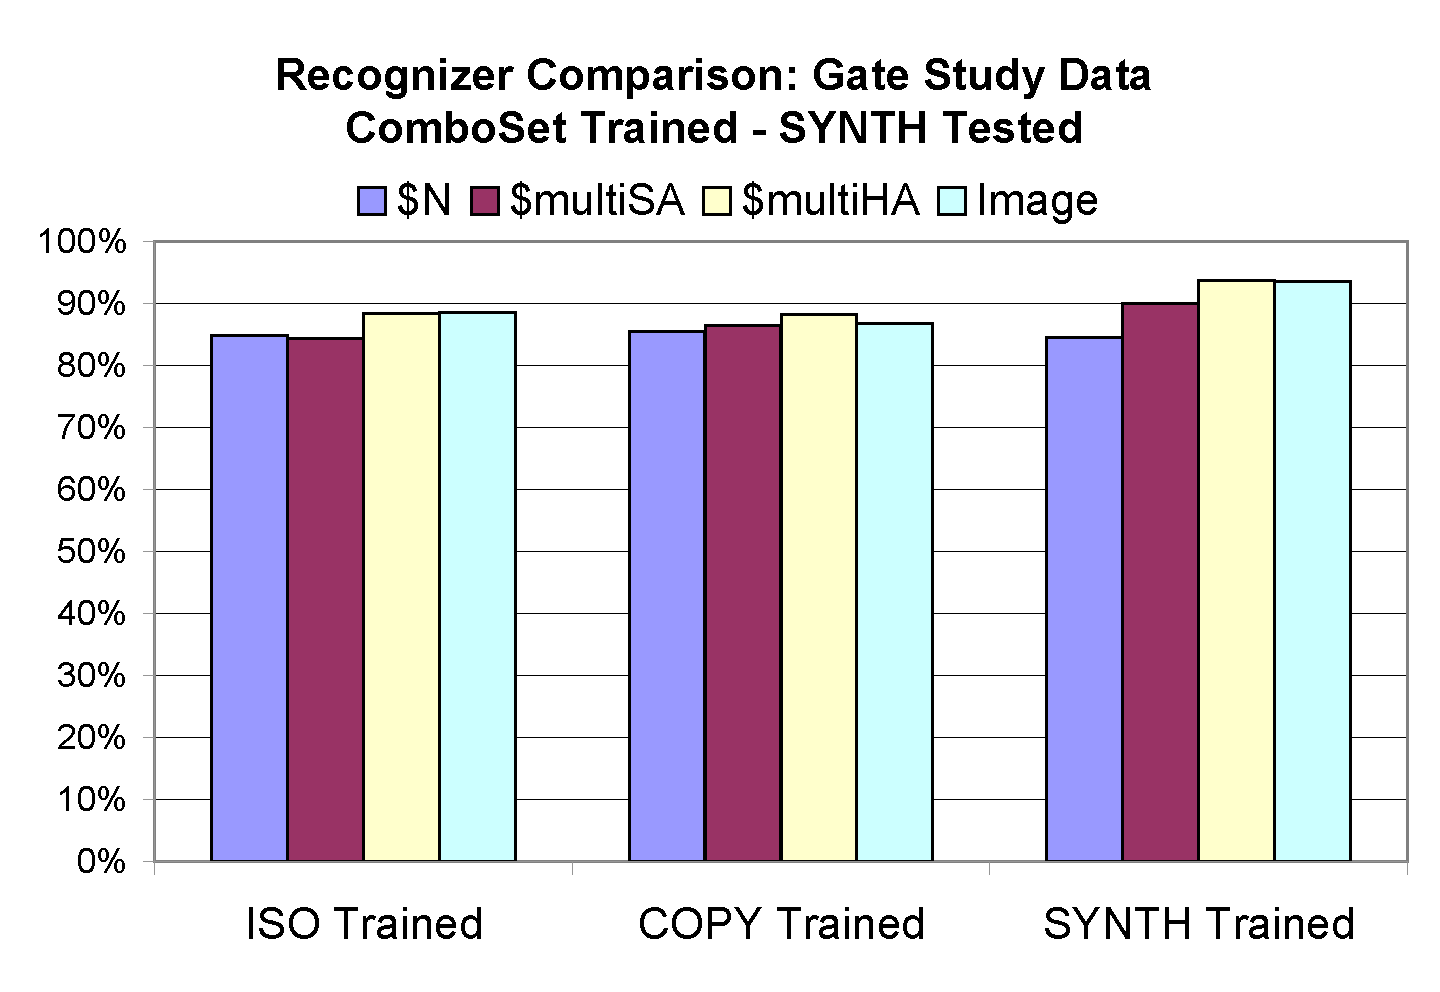
\includegraphics[width=\hsize]{RecComparisonGate.eps}
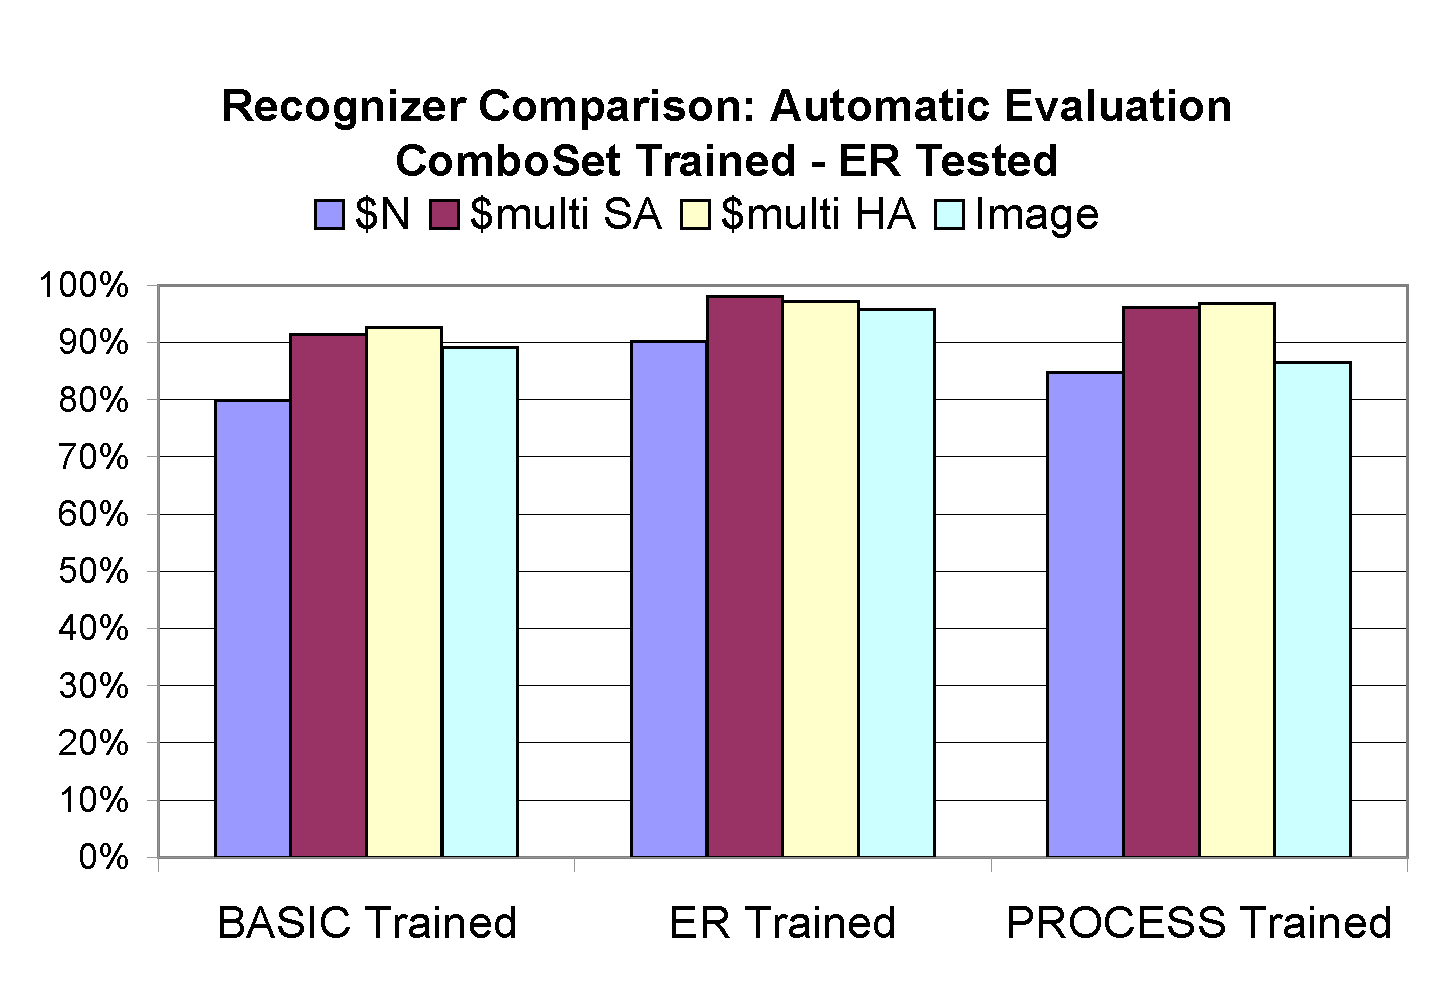
\includegraphics[width=\hsize]{RecComparisonAutoER.eps}
\includegraphics[width=\hsize]{RecComparisonAutoPROCESS.eps}
\end{center}
\caption{Performance comparison for the four recognizers used.  We trained the recognizers using the ComboSet method and tested them on SYNTH or SYNTH-like data.}
\label{RecComparison}
\end{figure}

In order to evaluate our new multi-dollar recognizer, we compare its performance to the \$N 
and Image-Based recognizers.  For this analysis, we use the same data we collected for the task-dependence and user-dependence experiments.  This allows us to compare our multi-dollar to \$N and the Image-Based recognizer in a number of different conditions.

For the \$N and Image-Based recognizers, we used optimal parameters as experimentally derived by the authors. We also performed some experimentation to determine optimal parameters for multi-dollar. We found no statistically significant improvement when increasing the points per shape above 48.  We came to the same conclusion when increasing the number of training examples.  We did not run any experiments decreasing either of these parameters below their initial values.

We used the same results from the trials explained in Sections~\ref{taskExperiment} and~\ref{userExperiment} to compile the results for this experiment.  We decided to focus on recognizers that were trained using the ComboSet approach, since that performed the best according to the experiments in Section~\ref{userExperiment}.  We also narrowed our scope to the SYNTH and SYNTH-like testing sets, because these represent the instances in which it is most important for the recognizers to perform well --- on real world data.  The results from these tests can be found in Figure~\ref{RecComparison}.

\begin{table}
\centerline{\begin{tabular}{|c|ccc|}
\hline
Comparison & ISO & COPY & SYNTH \\
\hline
MDHA and Image & 1.000 & 0.775 & 1.000\\
MDHA and MDSA&$\mathbf{<0.001}$ & $\mathbf{0.021}$ & $\mathbf{<0.001}$\\
MDHA and \$N &$\mathbf{<0.001}$ & $\mathbf{0.003}$ & $\mathbf{<0.001}$\\
Image and MDSA & $\mathbf{<0.001}$ & 1.000 & $\mathbf{<0.005}$ \\
Image and \$N & $\mathbf{<0.001}$ & 1.000 & $\mathbf{<0.001}$ \\
MDSA and \$N & 1.000 & 1.000 &  $\mathbf{<0.001}$ \\
 \hline
\end{tabular}}
\label{tab:recANOVA}
\caption{Repeated measures ANOVA test results comparing recognizer performance on circuit data.  Recognizers were trained with data from one of the three listed sets and tested on SYNTH data.  The recognizer listed first in each comparison is the one that performed better.}
\end{table}

We used a repeated measures ANOVA design to test, for each run, which recognizers performed significantly better than which other recognizers.  We used the Bonferroni post-hoc correction to reduce the chance of type 1 error.  A table of the results from running these tests on circuit data can be found in Table~\ref{tab:recANOVA}.  The multi-dollar Hungarian algorithm variant performs at least as well as the other three recognizers in every case, often outperforming other recognizers.  The results from the Automatic Evaluation data set are very similar, except that the multi-dollar simulated annealing variant performs almost as well as the Hungarian algorithm variant. This is likely because the 
Automatic Evaluation data set is primarily composed of single stroke shapes, so the simulated annealing search
is able to converge on the global minimum very quickly.

%-------------------------------------------------------------------------

\section{Discussion}
\label{discussion}


\subsection{The Effect of Task and User-Specific Data}
Our primary goal with this work was to determine whether data collected
using simpler isolated-shape data collection methods could be used
to train recognizers that would be applied to more complex synthesis tasks.
The answer to this question is mixed.  

We found that with a non-user-dependent recognizer, the task used to 
collect training data is not a very significant factor in recognition
performance. However, once a recognizer is augmented with user-specific
training, the additional benefit of task-specific training data becomes
apparent.  This result implies that while task-specific datasets are 
potentially useful in building free-sketch recognition systems, it is even 
more important to build recognition systems that allow users to train 
the systems to their own drawing styles using \emph{task specific training
examples.}  It is unlikely that users will be willing to hand group and label 
their own sketches for the benefit of the recognizer.  However, a system might 
leverage the error correction process
to collect additional training data: each time the user corrects a classification
error, the system can record this example and use it to train the 
recognizer.

The ``factory-trained, user-tuned'' recognizer framework has another advantage 
according to our results: we found that using a user semi-dependent training set
produced the best overall recognition results.  It is not surprising that including 
user-specific training data would improve recognition performance, but in many cases, 
using only user-specific training data actually \emph{decreased} performance.  We 
hypothesize that the ComboSet out-performs the UserSet in many cases because it is able 
to better handle within-user variation that we examined in Section~\ref{style} by including
a broader range of examples.  This hypothesis gains support when we look at the difference
between the two datasets.  With the Automatic Evaluation data, which is made up of 
very simple shapes, mostly drawn with one stroke, the ComboSet often did not out-perform
the UserSet.  With this simple data there is less room for within-user variation.


Overall, our results show the importance of using easily retrainable
recognizers for free-sketch recognition.  The multi-dollar and Image-Based
recognizers support online learning with very little effort or time
required. Furthermore, these recognizers need only a small number of
examples for training, requiring little extra work from the user to
benefit from increased recognition accuracy. However, there are many
recognizers for which it is not feasible to incorporate
user-dependence in a user-friendly way. For example, some recognizers
might need to rerun the entire training process, requiring a long
computation. Other recognizers might need to collect many examples
from a user before any effect on recognition would be noticed. 

We obtained our results on two data sets, and we expect that they would 
hold for other domains and other shapes, though more work is certainly needed to 
verify this claim.  In particular, each of our data sets included only a small number 
of shapes, so it is still an open question whether or not these trends would be 
different for a domain with more shapes.  Furthermore, although our data
simulates real-world tasks, it was still collected in a laboratory setting.
Actual real-world data might produce different trends, though we expect
that our trends would likely be more pronounced with real-world data
because that data is likely to be even more different from the isolated
shape data than the simulated 
real-world data produced in the laboratory.


\subsection{Comparison of Recognizers}
The multi-dollar recognizer, especially the Hungarian algorithm variant,
performed very well across the board.  We have also shown that the
simulated annealing version is a simpler alternative that still 
performs very competitively. Our modifications to the \$1 recognizer have
produced an easy-to-implement, highly accurate recognizer for symbol
recognition in freely-drawn sketches.

Our modified multi-dollar recognizer is actually quite similar to the
Image-Based recognizer. Both recognizers preprocess shapes by
rescaling and centering them, but where multi-dollar resamples points, the
Image-Based recognizer rasterizes points into a bitmap image. The next
step for both is a rotation search. However, because the Image-Based
recognizer performs its rotation search in polar coordinates, it must
also perform a separate distance calculation in screen coordinates
once the ideal angle has been located. To perform classification, both
recognizers compare the unknown symbol to each of the training
examples.

Although the general process is very similar for both recognizers, the
small differences have implications for how each performs. The
Image-Based recognizer is extremely robust to noise like overstroking,
touch-up strokes, or differing numbers of strokes in the unknown
symbol and the template. The modifications we made to the \$1
recognizer attempt to address touch-up strokes or differing numbers of
strokes in each shape. However, the resampling process includes the
endpoints of all strokes, so with more strokes, the points will be
poorly distributed, leading to an increased distance between the
unknown shape and template.

The advantage that multi-dollar has over the Image-Based
recognizer is its simplicity. We tried to stay as much in the spirit
of the original \$1 recognizer as possible. The simulated annealing
step requires only a small amount of extra code, but makes the recognizer
much more powerful than the original \$1.
The Hungarian algorithm adds more code
over simulated annealing, although it is a well-known
algorithm in the field of combinatorial optimization.
However, even with this added code, both versions of the multi-dollar recognizer
are simpler
than the Image-Based recognizer, especially the rotation search in
polar coordinates and the fact that our recognizer requires only one
distance metric rather than the four the Image-Based recognizer
requires.


%\subsection{Comparison of Data Sets}
%\note{We can probably work this into the previous section. 
%I think everything mentioned in this section has been covered in the previous
%comparison sections, I would say simply remove it. -Eric}

%In Sections~\ref{userExperiment} and~\ref{recExperiment}, we noted some 
%differences between the circuit data results and the Automatic Evaluation
%data results. In our recognizer comparison experiment (Section~\ref{recExperiment}),
%we found that multi-dollar with simulated annealing performed almost as
%well as the Hungarian algorithm variant, unlike with the circuit data. 
%This result is likely because the Automatic Evaluation data is comprised of 
%mostly single-stroke symbols, which make it easier for simulated annealing
%to converge on the correct solution.  More generally, there may
%be some domains in which the simpler simulated annealing version performs
%just as well as the Hungarian algorithm.  

%-------------------------------------------------------------------------
\section{Conclusion}

We have shown that using user-specific training data in addition to global 
training data provides a significant advantage to using only global training
data. Our experiments suggest that drawing style (stroke order) is moderately consistent within and across tasks. However, in the user semi-dependent and user-dependent training conditions, the best
recognition accuracy is attained via task-specific training data.  Finally,
we have introduced an extremely accurate recognizer for symbols drawn in 
free-sketches and a simpler alternative that sacrifices a small amount of 
performance for ease of implementation.


%\note{this needs an overhaul}
%We have shown that it is possible to train a highly accurate
%recognizer using only isolated shapes as training data. This is
%important because isolated shape data is much easier to collect than
%naturally drawn shapes. It is also much easier to group and label
%isolated shapes than complicated diagrams.  We have also shown that
%whenever possible, user-specific examples should be incorporated into
%training. For classifiers like the Image-Based and multi-dollar recognizers
%that support online learning, user-specific examples are an easy way
%to improve accuracy.

%-------------------------------------------------------------------------

\bibliographystyle{elsarticle-num}

\bibliography{gatestudy}

\end{document}
